\chapterimage{/6/head2.jpg} % Chapter heading image
\chapter{Un universo... Perturbato}\label{6:ch}

\section{Formazione delle strutture cosmiche}
La trattazione che segue deriva dalla teoria perturbativa: ossia il campo di densità non si considera perfettamente omogeneo, ma si introducono delle piccole perturbazioni e se ne studia l'evoluzione a partire dalle leggi già studiate. Queste fluttuazioni possono essere originate dall'inflazione. Sono state osservate nel 1991 dal satellite COBE come $\delta T / T \sim 10^{-5}\leftrightarrow \delta \rho / \rho$ (assumendo adiabaticità) a $z=1100$ e come $\delta \rho /\rho \sim 10^{2\div 3}$ attraverso la struttura a grande scala a $z=0$.

Esiste una scala fisica (detta \textit{di Jeans}) oltre la quale si ha il collasso gravitazionale e si ottiene ponendo:

\begin{example}[$\mathbf{E_{kin}=E_{pot}}$]
    $R_J \propto v \sqrt{\frac{1}{2 G \rho}} $
\end{example}
\begin{example}[$\mathbf{\bar{F}_{press}=\bar{g}}$]
    $R_J \propto v_s \sqrt{\frac{1}{G \rho}} $
\end{example}
\begin{example}[$\mathbf{\tau_{free\, fall}=\tau_{sound\, crossing}}$]
        $R_J \propto v_s \sqrt{\frac{1}{2 G \rho}} $
\end{example}
In ambetrè i casi ci sono due processi in competizione: da una parte la gravità, dall'altra la dispersione di velocità / pressione / attraversamento. 
Per scale $R>R_J$ si ha collasso gravitazionale, per quelle più piccole la perturbazione si dissolverà.

%\begin{theorem}[Principio dell'instabilità gravitazionale]
%Piccole perturbazioni crescono.
%\end{theorem}

\section{Teoria di Jeans classica}
Il metodo consiste nell'applicare piccole perturbazioni ad uno stato di equilibrio stazionario, omogeneo e isotropo. Soluzioni analitiche si possono trovare solamente in regime lineare e verranno espresse sotto forma di serie di Fourier. Le equazioni fondamentali sono: conservazione della massa, del momento (Eulero) ed equazione di Poisson, a queste si aggiunge un'equazione di stato:
\begin{equation}\left\{
    \def\arraystretch{1.5}
        \begin{array}{l}
        \rho_t + \nabla \rho \cdot \vec{v} + \rho \nabla \cdot \vec{v} =0\\
        \rho \left (  \vec{v}_t + (\vec{v}\cdot \nabla )\vec{v}\right)=-\nabla p + \rho \nabla \phi \\
        \nabla^2 \phi = -4\pi G \rho \\
        p=p(\rho, S) 
    \end{array}\right. \label{eq:6planksys}
\end{equation}
ove il pedice indica la derivazione parziale rispetto al tempo. 

Si considereranno, così come corroborato dalle osservazioni, solamente soluzioni adiabatiche: $p(\rho, S)\rightarrow p(\rho)$. Lo stato di equilibrio si introduce ipotizzando che le costanti $\rho_0$, $p_0$, $\phi_0$ (``di background'') soddisfino il sistema (\ref{eq:6planksys}). In realtà questa soluzione non è ammissibile fisicamente poiché $\phi_0 = cost \Leftrightarrow \rho_0=0 $, ma è comunque didattica. Lo stesso non si verificherà quando saranno considerate le soluzioni di Friedmann $\rho_0(t)$, $\phi_0(t)$, $v_{exp}$.

Il sistema linearizzato che governa le piccole perturbazioni, sapendo che $c_s^2 = \left . \frac{\partial p}{\partial \rho} \right |_{S=cost}$, è:
\begin{equation}\left\{
    \def\arraystretch{1.5}
        \begin{array}{l}
        \delta\rho_t + \rho_0\nabla\cdot \delta \vec{v} =0 \\
        \rho_0 \left ( \delta \vec{v}_t + c_s^2 \nabla \delta - \nabla \delta\phi \right) = 0 \\
        \nabla^2 \delta \phi = -4\pi G \delta\rho
    \end{array}\right. 
\end{equation}
ove $\delta=\delta \rho / \rho_0$ e per $\delta \rho_t$ si intende $(\delta\rho)_t$. Si nota che i termini dipendenti solamente dalle quantità di backgruond si semplificano poiché soddisfano le equazioni del sistema (\ref{eq:6planksys}).

Si cercano soluzioni/perturbazioni separate nella dipendenza spazio-tempo nello spazio di Fourier: $S(\vec{r},t)=S_k \: e^{i(\vec{k}\cdot\vec{r}-\omega t)}$. Per cui valgono le relazioni: $S_t = -i\omega S$, $\nabla S = i\vec{k}S$ e $\nabla^2 S= -k^2 S$ e nella direzione longitudinale al moto ($\vec{k}\cdot\vec{v}=kv$) si ottiene il seguente sistema di dispersione:
\begin{equation}\left\{
    \def\arraystretch{1.5}
        \begin{array}{l}
        - \omega \delta_k + k \delta v_k = 0 \\
        - \omega \delta v_k + k (c_s^2\delta_k -\delta\phi_k) = 0 \\
        - k^2 \delta\phi_k = -4\pi G\delta\rho_k
    \end{array}\right. 
\end{equation}
che definisce la relazione tra l'ampiezza dell'onda del contrasto di densità con l'ampiezza dell'onda del contrasto di velocità (ora i pedici non indicano più una derivazione, ma la dipenza da $k$). Questo è reso più evidente dall'\textbf{equazione di dispersione} che si ottiene annullando determinante del sistema:
\begin{equation}
    \omega^2 = c_s^2 k^2 - 4\pi G \rho_0 \label{eq:6disprelstatic}
\end{equation}

Per $\omega^2 < 0 \rightarrow \omega \in \mathbb{C}$ si hanno due soluzioni esponenziali: una crescente e una decrescente. Per $\omega^2 > 0 \rightarrow \omega \in \mathbb{R}$ si hanno due onde di piccola ampiezza logitudinali con verso opposto. Con la condizione $\omega^2 = 0$ vengono definiti il \textit{numero d'onda di Jeans} e la \textit{lunghezza d'onda di Jeans} ($\lambda=2\pi /k$, che verrà spesso chiamata \textit{scala di Jeans}):
\begin{equation}
k_J = \sqrt{\frac{4\pi G \rho_0}{c_s^2}} \qquad \lambda_J=c_s\sqrt{\frac{\pi}{G\rho_0}} \qquad \omega^2=k^2 c_s^2 \left[1- \left(\frac{\lambda}{\lambda_J}\right)^2\right]
\end{equation}

Quindi ricapitolando si ha:
\begin{itemize}
    \item $\lambda >\lambda_J$ oppure $k<k_J$: $\delta = \delta_k e^{\mp |\omega| t}e^{ikr} $ onda con stessa forma spaziale, ma ampiezza che dampa o esplode. Quest'ultimo caso (crescente) è quello interessante da un punto di vista cosmologico.
    \item $\lambda <\lambda_J$ oppure $k>k_J$: la perturbazione rimane sotto forma di due onde, una receding e una proceding, di ampiezza costante.
    \item $\omega^2=0$ è come se l'onda si congelasse ($v_{fase}=0$)
\end{itemize}

\vspace{1em}
\noindent Questa trattazione vale fintantoché $\delta \ll 1$ (osservativamente i galaxy clusters arrivano anche a $1000$). Inoltre, includendo l'effetto dell'espansione dell'universo ci si aspetta una crescita delle perturbazioni più lenta di quella esponenziale.


\newpage
\section{Teoria di Jeans cosmologica}
Per la trattazione cosmologica è necessario considerare tre scale fondamentali:
\begin{enumerate}
    \item $R_H$ discrimina le scale sotto cui va considerata la microfisica, per $R>R_H$ l'unica interazione fondamentale da considerare è la gravità;
    \item $R_J$ sarà rilevante solo se $<R_H$;
    \item $R_d$ ossia la scala di dissipazione delle onde (differente per la materia ordinaria e quella oscura).
\end{enumerate}
Le prime due sono evidentemente variabili nel tempo.

Entrano poi in gioco due tempi fondamentali:
\begin{enumerate}
    \item $t_{equivalence}$ discrimina la dominanza di radiazione/materia;
    \item $t_{decoupling}$ la pressione di radiazione impedisce il collasso della materia se accoppiata, inoltre come si è visto (?): $t_{dec,DM} < t_{eq} < t_{rec,b}$.
\end{enumerate}

Si utilizzano le equazioni di Friedmann considerando la perturbazione come un piccolo universo chiuso immerso in un universo di background meno denso e piatto (per semplificare i conti). La soluzione è relativistica, ma in questo caso si sta considerando solamente la gravità, per cui sarà valida per: scale maggiori di $R_H$ o minori di $R_H$, ma sufficiendemente più grandi della $R_J$. 

Tramite la prima equazione di Friedmann si ha rispettivamente per perturbazione e background:
\begin{equation}\left\{
    \def\arraystretch{1.5}
        \begin{array}{l}
            H_p^2=\frac{8\pi }{3}G \rho_p - \frac{c^2}{a^2}\\
            H_b^2 =\frac{8\pi}{3}G \rho_b
    \end{array}\right. \quad\leftrightarrow\quad \delta \propto \left(\rho_b a^2\right)^{-1}\propto a^{1+3w}\propto
    \left\{
   \begin{array}{ll}
        a^2 & t<t_{eq}\\
        a & t>t_{eq}
\end{array}\right. 
\end{equation}
dove si sono sincronizzati gli universi ponendo $H_p=H_b$.

\subsection{Soluzione per $\mathbf{R > R_H}$}
Fuori dall'orizzonte solo la gravità domina le cose, le altre componenti seguono la gravità, pertanto:
\begin{equation}
    \def\arraystretch{1.3}
        \begin{array}{ll}
            t<t_{eq} & \delta_m \to  \delta_r \propto a^2  \\
            t>t_{eq} & \delta_r \to \delta_m \propto a  
    \end{array} \label{none}
\end{equation}
Le perturbazioni crescono tutte in modo uguale e le componenti sottodominanti seguono quella dominante.

\begin{theorem}[Messaggio da portare a casa]
Fuori dall'orizzonte le perturbazioni crescono sempre, ma con un andamento che cambia a $t_{eq}$. Prima seguono l'andamento della radiazione, dopo quello della materia. Attenzione però: $R_H=R_H(t)$.
\end{theorem}


\subsection{Soluzione per $\mathbf{R < R_H}$}\label{ch6:chilovoleva}
Per trovare le soluzioni all'interno dell'orizzonte bisogna tener conto dell'espansione dell'universo. Le coordinate che contano sono quelle fisiche ($r$) , ma passando alle coordinate comoventi ($x$) si possono semplificare i conti: $r=a/a_0 \; x$, di solito $a_0=1$. Si può dimostrare che $\d{r}/\d{t} = Hr + a\dt{x} = Hr+ v_{pec}$. La $v_{pec}$ sarà la perturbazione rispetto al flusso di Hubble, dovuta alla disomogeneità della materia. Utilizzando $u=\dt{r}$, si può riscrivere il sistema per il modello fisico:
\begin{equation}\left\{
    \def\arraystretch{1.5}
    \begin{array}{l}
        \rho_t + \nabla\cdot (\rho \vec{u}) =0 \\
        \rho \left ( \vec{u}_t + (\vec{u} \cdot \nabla) \vec{u} \right) = -\nabla p +\rho \nabla \phi \\
        \nabla^2 \phi = - 4 \pi G \rho
    \end{array}\right.
\end{equation}
In questo caso si cercano soluzioni del tipo: $\rho = \rho_0 (1+\delta)$, $u=Hr+v_{pec}$, $\phi=\phi_0+\delta\phi$ e $p=p_0+\delta p$. Il sistema linearizzato che governa le piccole perturbazioni diventa:
\begin{equation}\left\{
    \def\arraystretch{1.5}
    \begin{array}{l}
        \delta\rho_t + \rho_0 \nabla\cdot\vec{v}_{pec} + 3H \delta\rho + Hr \nabla \delta\rho \cdot \hat{r} =0 \\
        \rho_0 \left ( \vec{v}_{pec, t} + H \vec{v}_{pec}+ Hr\nabla\vec{v}_{pec}\right ) = -c_s^2 \nabla\delta\rho +\rho_0\nabla\phi \\
        \nabla^2 \delta \phi = -4\pi G \delta\rho
    \end{array}\right.
\end{equation}

A questo punto si cambia il sistema di riferimento in coordinate comoventi per ``riassorbire'' l'espansione dell'universo (le coordinate comoventi non dipendono dal tempo). In particolare gli operatori diventano:
\begin{equation*}
    \def\arraystretch{1.5}
    \begin{array}{l}
        \nabla_r = \frac{1}{a}\nabla_x \\
        \frac{\d{f}}{\d{t}} = \left. \frac{\partial}{\partial t} \right|_r f + Hr \nabla_r f = \left. \frac{\partial}{\partial t} \right|_x f + 0 \qquad \rightarrow \qquad \left. \frac{\partial}{\partial t} \right|_r f = \left. \frac{\partial}{\partial t} \right|_x f - Hr \nabla_r f  
    \end{array}
\end{equation*}
Quindi il sistema in coordinate comoventi diventa:
\begin{equation}\left\{
    \def\arraystretch{1.5}
    \begin{array}{l}
        \delta\rho_t + \frac{\rho_0}{a} \nabla \cdot\vec{v}_{pec} + 3H \delta\rho =0 \\
        \rho_0 \left ( \vec{v}_{pec, t} + H \vec{v}_{pec} \right) = -\frac{c_s^2}{a} \nabla\delta\rho +\frac{\rho_0}{a}\nabla\phi \\
        \frac{1}{a^2}\nabla^2 \delta \phi = -4\pi G \delta\rho 
    \end{array}\right.
\end{equation}

Si  cercano  soluzioni/perturbazioni  nello  spazio  di Fourier nella forma: $S(r,t) =S_k (t)\: e^{ikx}$, poiché già si sa che le ampiezze dipenderanno dal tempo. Includendo l'evoluzione  si ottiene il seguente sistema di dispersione: 

\textbf{Dopo l'equivalenza} il background è dominato dalla materia, per cui: $\rho_0 \propto a^{-3}$, $p_{rad}=0$.
\begin{equation}\left\{
    \def\arraystretch{1.5}
    \begin{array}{l}
        \dt{\delta}_{k} + \frac{i\vec{k}\cdot\vec{v}_k}{a}=0 \\
        \dt{\vec{v}}_k + H \vec{v}_k = -\frac{i\vec{k}}{a}\left( v_s^2 \delta_k + \delta\phi_k\right) \\
        \delta\phi_k = \frac{4 \pi G \delta \rho_k a^2}{k^2}
    \end{array}\right.
\end{equation}
dove per alleggerire la notazione si è utilizzato il punto per le derivate temporali e $v=v_{pec}$. A questo punto si scompone il campo di velocità lungo la terna ortonormale del vettore d'onda \{$\hat{n}$, $\hat{t}_1$, $\hat{t}_2$\} dove la prima componente rappresenta la direzione longitudinale / parallela a $\vec{k}$ e le altre due formano il piano perpendicolare ad essa. In questo modo si ha:
$$
\vec{v}_k = \vec{v}_{k,\perp} + \vec{v}_{k,\parallel} \qquad \rightarrow \qquad \nabla \cdot \vec{v}_{k,\perp} = 0; \quad \nabla \times  \vec{v}_{k,\parallel} =0
$$

L'equazione di Eulero per la componente perpendicolare si riduce a $\d{( a\vec{v}_{k,\perp})}/\d{t}=0 \rightarrow \vec{v}_{k,\perp}\propto a^{-1}$. Questo significa che, se l'universo si espande, l'eventuale componente rotazionale del campo di velocità decresce nel tempo e si può quindi trascurare.
Aggiornando il sistema per la componente longitudinale e svolgendo le dovute operazioni cosmatematiche (tra cui riportare le coordinate al sistema fisico $k/a\rightarrow k$) si ottiene l'\textbf{equazione di dispersione} per il modello in esame:
\begin{equation}
    \ddt{\delta}_k + 2 \frac{\dt{a}}{a}\dt{\delta}_k + \delta_k \left( k^2 c_s^2 -4\pi G \rho_0\right) =0 \label{eq:6disprelmat}
\end{equation}
La quale per un universo statico (derivate temporali nulle) si riconduce all'equazione (\ref{eq:6disprelstatic}).

La cosmologia è nascosta in $\dt{a}/a$ e in $\rho_0$ nella relazione tra redshift e tempo.


\subsubsection{Universo EdS di sola materia}
Applicando le relazioni ricavate nel paragrafo \ref{6:chsub:eds} si cercano soluzioni nella forma $\delta_k \propto t^\alpha$:
\begin{equation*}
3\alpha^2 + \alpha + 2\left( \frac{k^2 c_s^2}{4\pi G \rho_0}-1\right)=0
\end{equation*}
Il valore che annulla il discriminante è $k_J= \sqrt{25\pi G \rho_0 /6c_s^2}$. Si hanno due soluzioni reali ($\Delta >0$, $k<k_J$, $\lambda >\lambda_J$) se:
\begin{equation*}
\alpha_{1,2}=-\frac{1\pm 5\sqrt{1-\left( \lambda_J /\lambda\right)^2}}{6}
\end{equation*}

La soluzione interessante è quella crescente, che dipende da quanto la lunghezza d'onda delle perturbazioni è vicino a quella di Jeans.
Per $\lambda \gg \lambda_J$ (si può trascurare il termine con $c_s$ rispetto a quello gravitazionale) si ha:
\begin{equation}\delta_k \propto  \left\{
    \def\arraystretch{1.5}
        \begin{array}{ll}
            t^{-1} & trascurabile \\
            t^{2/3} \propto a & 
    \end{array}\right. 
\end{equation}

Ossia le perturbazioni negli universi EdS in regime lineare per scale molto più grandi di quella di Jeans crescono come il fattore di espansione. Per scale più vicine a $\lambda_J$ ci si aspetta un rallentamento dovuto agli effetti di interazione del fluido fino ad arrivare ad uno stato stazionario. Si ricorda che tutto questo vale dopo il disaccoppiamento dalla radiazione, momento che avviene prima per la materia oscura rispetto a quella barionica.

\subsubsection{Universo Curvo di sola materia}
Svolgendo la derivata seconda di $H=\dt{a} / a$, inserendo la seconda equazione di Friedmann per la materia e derivando ulteriormente si ha:
\begin{equation*}
    \ddt{H}+2H\dt{H}-4\pi G \rho_0 H = 0 \qquad vs. \qquad (6.12) \quad \ddt{\delta}_k + 2 \frac{\dt{a}}{a}\dt{\delta}_k + \left( k^2 c_s^2 -4\pi G \rho_0\right) \delta_k  =0
\end{equation*}

Per $\lambda \gg \lambda_J$ il termine con $c_s^2$ è trascurabile, pertanto ci si aspetta che le soluzioni siano le stesse ottenute in precedenza con $\delta_k \rightarrow H$. Quando si sono cercate le soluzioni all'equazione di Friedmann è stata imposta l'espansione dell'universo, scegliendo formalmente una delle due possibili soluzioni. Questa, mediante l'analogia, corrisponderebbe alla soluzione decrescente ($\delta_- \propto t^{-1}$), ossia quella meno intrigante. Ancor meno intrigante è il teorema del Wronskiano $W$, che ci consente, avendo due signore funzioni (derivabili, ecc..) di ottenere la soluzione crescente:
$$
y''+Py'+Qy=0 \qquad W=y_1'y_2 - y_1y_2'; \; W'=-PW \quad \rightarrow \quad W=\delta_-\dt{\delta}_+ - \dt{\delta}_-\delta_+ \propto a^{-2}
$$
Integrando il differenziale del rapporto tra $\delta_+$ e $\delta_-$ si ottiene la relazione tra le due soluzioni:
\begin{equation*}
    \delta_+ = \delta_- \int \frac{\delta_-\dt{\delta}_+ - \dt{\delta}_-\delta_+}{\delta_-^2}\d{t}\quad\propto\quad \delta_- \int \frac{\d{t}}{\delta_-^2\: a^2}
\end{equation*}
Essendo $\d{z}=-H(1+z)\d{t}$ si ottiene l'evoluzione del cosiddetto \textbf{growing factor}:
\begin{equation}
    \delta_+ = -\frac{H(z)}{a_0^2}\int \frac{1+z}{H^3}\d{z}
\end{equation}
In generale questo integrale non ha soluzione analitica (si ricorda che $H=H_0 E$). Nei modelli EdS la crescita va come $a\propto (1+z)^{-1}$, ci si aspetta una crescita inferiore negli universi aperti e una crescita superiore in quelli chiusi (nei quali diminuisce il termine di ``frizione'' dovuto all'espansione).

\begin{figure}[H]
    \centering
    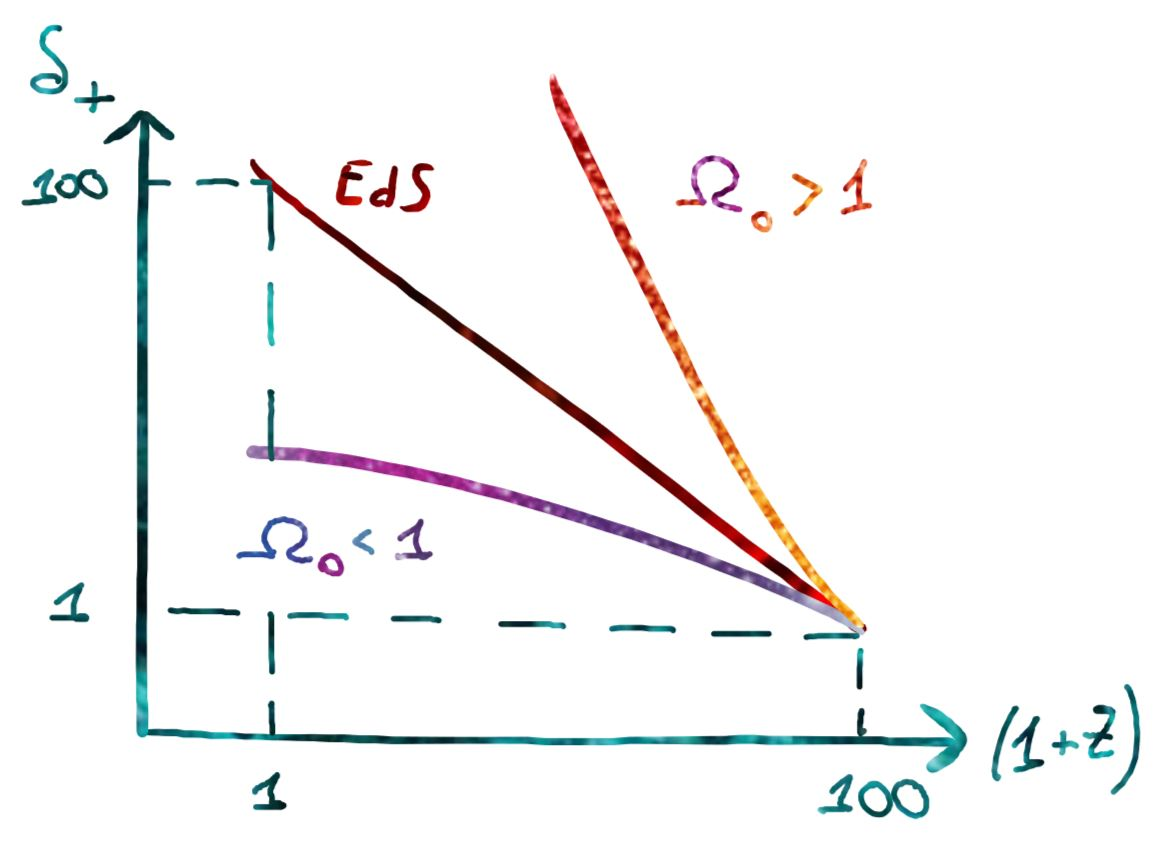
\includegraphics[width=.6 \textwidth]{Pictures/6/crescitapertmat.jpg}
    \caption{Evolzione delle perturbazioni per universi chiusi, EdS e aperti di sola materia. Queste considerazioni valgono quindi per $t>t_{eq}$ e in realtà per $\delta \ll 1$. Attenzione: normalizzando le curve a oggi gli andamenti di universi aperti e chiusi si scambiano sopra-sotto, inoltre non è garantita la correttezza delle concavità. }
\end{figure}

In realtà esiste una relazione pseudo-analitica che fa uso di $f=\d{\ln \delta_+} / \d{\ln a}$ per riscalare la crescita:
\begin{equation*}
    f=\Omegam^{0.55} - \frac{\OmegaL}{70} (1+\Omegam /2)
\end{equation*}

All'aumentare della materia le perturbazioni crescono più velocemente, mentre la costante cosmologica è meno influente. Per $\Omegam=1$ si recupera l'andamento $\delta_+ \propto a$. Il numero $0.55$ è magico poiché è una delle predizioni precise della relatività generale. Osservando la variazione del fattore di crescita al variare di $\Omegam$ si può falsificare la teoria della relatività generale. Altrimenti assumendola buona, si possono porre constraints sulla cosmolgia (conteggio ammassi al variare di z, tomografia weak lensing).

\vspace{1em}
Fluttuazioni nella desità sono state osservate come $\delta T /T \sim 10^{-5}$ nella CMB ($z\sim 10^3$). Utilizzando le relazioni trovate in regime lineare, ci si aspetterebbe: $\delta (z=0) \sim 10^{-2}$ contrariamente a quanto osservato $\delta_{obs} (z=0)\sim 100$ (regime chiaramente non linerare). Ragionando in modo opposto, si fissa $\delta (z=0) = 1 $ (ipotizzando che sia diventato $\sim 100$ ieri l'altro), questo richiede che $\delta_{CMB}\sim 10^{-3}$. Un modo per giustificare il fatto che non si osserva è ricorrere agli universi chiusi, ma servirebbe $\Omega \approx 10$ (alèèè, un pò troppo chiuso!). La soluzione è che attorno ai barioni vi è una distribuzione di DM non più uniforme (avviene come si vedrà il \textit{barion ``ketchup''}). Questa può anche essere vista come una delle prove a favore dell'esistenza della DM, che aiuta a far crescere le perturbazioni essendosi disaccoppiata prima.
\vspace{1em}


\subsubsection{Universo EdS di sola radiazione}
\textbf{Prima dell'equivalenza} non si può trascurare il contributo della pressione di radiazione, per cui nelle equazioni del sistema (\ref{eq:6planksys}) va fatta la sostituzione $\rho \rightarrow \rho + 3p/c^2$ ($c_s=c/\sqrt{3}$). Analogamente a come si è fatto in precedenza: si ipotizza che esista una soluzione imperturbata data dall'espansione dell'universo, si aggiunge una piccola perturbazione e si linearizzano le equazioni. Si ottiene la seguente \textbf{equazione di dispersione}:
\begin{equation}
    \ddt{\delta}_k + 2 \frac{\dt{a}}{a}\dt{\delta}_k + \delta_k \left( k^2 c_s^2 -\frac{32}{3}\pi G \rho_0\right) =0
\end{equation}

Applicando le relazioni per un universo EdS di sola radiazione (Paragrafo \ref{6:chsub:eds}, $w=1/3$) si cercano soluzioni sotto forma di $\delta_k \propto t^{\alpha}$:
\begin{equation*}
    \alpha^2 = 1-\frac{3k^2c_s^2}{32 \pi G\rho_0}
\end{equation*}
Pertanto si definisce: $k_J=\sqrt{32\pi G \rho_0 / 3c_s^2}$. Si hanno due soluzioni reali ($\alpha^2=0$, $\lambda >\lambda_J$) se:
\begin{equation*}
    \alpha_{1,2}=\pm \sqrt{1-\left( \lambda_J /\lambda\right)^2}\qquad \rightarrow \qquad \alpha_{1,2}=\pm 1 \quad per\; \lambda \gg \lambda_J
\end{equation*}

La dipendenza interessante è quindi $\delta_k \propto t^1$ a differenza dell'andamento $t^{2/3}$ per la materia, ossia dopo l'equivalenza. Il problema sta nel capire quanto è grande la scala di Jeans rispetto alla scala dell'orizzonte. La relazione di dispersione può essere riscritta nella forma: $1-k_J^2c_s^2t^2 = 0$, ossia ($c_s=c/\sqrt{3}$): 
\begin{equation*}
    k_J = \sqrt{3}/ct \qquad\rightarrow \qquad \lambda_J = 2\pi c t /\sqrt{3} \quad > \quad R_H = 2ct
\end{equation*}

La scala di Jeans è quindi più grande della scala dell'orizzonte: il problema sta nel fatto che la scala di Jeans non sta dentro l'orizzonte e non ha quindi senso fisico (fuori dall'orizzonte le perturbazioni crescono sempre, non hanno una scala). Questo significa che \textbf{non c'è la possibilità di far crescere le perturbazioni durante l'era radiativa}. Inoltre, il fatto che le perturbazioni si stiano propagando così velocemente, fa si che mediamente $\delta_r =0$ e di conseguenza tutte le altre componenti accoppiate. Tradotto in altro modo, la pressione di radiazione è talmente forte che impedisce il collasso.

\subsubsection{Materia oscura}
Per la dark matter vale l'equazione di dispersione (\ref{eq:6disprelmat}), che deve essere riadattata tenendo conto dell'epoca radiativa. In particolare $c_s^2$ diventa la pressione/dispersione di velocità della DM e nel termine gravitazionale bisogna considerare tutte le componenti: $\rho_0 \delta_k \rightarrow \rho_r\delta_r + \rho_{b}\delta_{b} + \rho_{DM}\delta_{DM} $. La prima è trascurabile poiché, come appena visto, non ci sono contrasti nella componente relativistica e pure la componente barionica poiché è ad essa accoppiata. L'\textbf{equazione di dispersione} diventa:
\begin{equation}
    \ddt{\delta}_{k,DM}+ 2 \frac{\dt{a}}{a}\dt{\delta}_{k,DM} + \left( k^2 c_s^2 -4\pi G \rho_{0,DM}\right)\delta_{k,DM}  =0
\end{equation}

Ancora una volta si cercano soluzoni per $\lambda \gg \lambda_J$. È conveniente cambiare variabile utilizzando $x=a/a_{eq}\rightarrow \frac{\d{}}{\d{t}}=\frac{\dt{a}}{a_{eq}}\frac{d{}}{\d{x}}\rightarrow \frac{\d{}^2}{\d{t^2}}=\frac{\ddt{a}}{a_{eq}}+\frac{\d{}}{\d{x}}+\left(\frac{\dt{a}}{a_{eq}}\right)^2 + \frac{\d{}^2}{\d{x^2}}$. In seguito si inserisce l'evoluzione delle densità in funzione di $a$, in particolare: $\rho_{DM} (a) / \rho_r(a) = x$. Per eliminare le dipendenze da $\dt{a}$ e $\ddt{a}$ si utilizzano infine le rispettive equazioni di Friedmann, dove la densità è data da $\rho_{DM}+\rho_{r}$ e la pressione $p_{DM}+p_r$:
\begin{equation*}
    \rho_{DM}=\frac{3H^2 x}{8\pi G (1+x)}; \qquad \frac{\dt{a}}{a_{eq}}=Hx; \qquad \frac{\ddt{a}}{a_{eq}}=-\frac{x(x+2)H^2}{2(x+1)};   
\end{equation*}
Con un po' di \textit{maquillage} si ottiene:
\begin{equation}
    \delta_{k,DM}'' + \frac{3x+2}{2x(1+x)}\delta_{k,DM}' - \frac{3}{2x(1+x)}\delta_{k,DM}=0
\end{equation}
Dove l'apice indica la derivata rispetto a $x$. Questa è un'equazione ipergeometrica che ha come soluzione crescente: $\delta_{k,DM}^+ = 1+3x/2$ valevole entro l'orizzonte solo prima dell'equivalenza, in particolare:
\begin{equation}
    \frac{\delta (t_{eq})}{\delta(t_H)}=\frac{1+3/2}{1+3a_H/2a_{eq}} \quad < \quad 5/2
\end{equation}

Questo rappresenta il fattore di crescita delle perturbazioni di materia oscura dal momento in cui queste entrano nell'orizzonte fino al momento per cui la soluzione è valida (il tempo dell'equivalenza). L'entrata nell'orizzonte può avvenire al più quando $a_H\rightarrow 0$ (un istante dopo il BB). Dopo l'equivalenza la crescita riprende con le leggi già viste. 

\begin{definition} 
Le perturbazioni di DM dentro l'orizzonte possono crescere fino a $t_{eq}$ al più di un fattore $5/2$ (una cavolatina). Questo viene detto \textbf{effetto di stagnazione} o \textbf{effetto Meszaros}. In altri termini, nell'epoca dominata dalla radiazione il tempo scala di espansione dell'universo è minore del tempo scala di collasso delle perturbazioni di DM (il campo dominante, quello radiativo, non ha fluttuazioni).
\end{definition}

La teoria lineare lontano dalla $\lambda_J$ non prevedeva una dipendenza dalla scala, che viene invece introdotta dall'effetto Meszaros. Le scale che sono potute entrare nell'orizzonte prima dell'equivalenza sono infatti modificate (Fig. \ref{fig6:mezaros}). 


\begin{figure}[H]
    \centering
    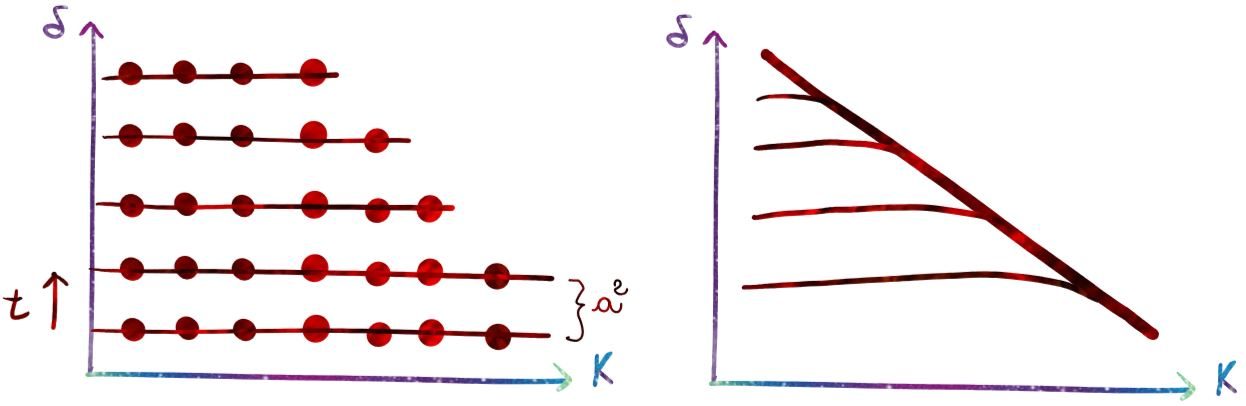
\includegraphics[width= .93 \textwidth]{Pictures/6/meszarus.jpg}
    \caption{Sinistra: Si suppone che inizialmente le perturbazioni nascano tutte uguali, indipendente da $k$ (in realtà non sarà così). Ogni punto rappresenta discretamente una perturbazione sulla scala $k$. Fuori dall'orizzonte le perturbazioni crescono come $a^2$ indipendentemente dalla scala. La prima scala ad entrare nell'orizzonte è quella con $\lambda$ più piccolo, ossia con $k$ più grande. I punti che entrano nell'orizzonte stagnano, pertanto l'altezza delle perturbazioni non è più costante e viene introdotta una dipendenza da $k$. L'evoluzione cumulativa è mostrata nella figura a destra. Dopo l'equivalenza, la crescita torna ad essere indipendente da $k$, quindi si formeranno curve autosimilari.}\label{fig6:mezaros}
\end{figure}


\subsection{Fluttuazioni barioniche}
I poveri barioni hanno la sfortuna/fortuna di essere accoppiati alla radiazione fino a $z\sim 1000$.  Vorrebbero fare gravità e collassare, ma la pressione di radiazione lo impedisce ed essi oscillano. In seguito alla ricombinazione dell'idrogeno il barione si accorge di esser tale, ma nel frattempo la materia oscura, disaccoppiandosi prima, ha potuto fare i suoi porci comodi. Per questo motivo i barioni si trovano le buche di potenziale della materia oscura già belle che formate. Inizialmente, il contrasto di densità dei barioni risponde a un capo gravitazionale prodotto dalla DM e l'\textbf{equazione di dispersione} è:
\begin{equation}
    \ddt{\delta}_{k,b}+ 2 \frac{\dt{a}}{a}\dt{\delta}_{k,b} + \left( k^2 c_s^2 -4\pi G \rho_{0,DM}\right)\delta_{k,DM}  =0
\end{equation}

Assumendo un universo EdS $\delta_{k,DM}=Aa$, indicando con l'apice la derivata rispetto ad $a$ e utilizzando le equazioni di Friedmann come nel conto precedente (qui $\rho_{DM}\gg\rho_{b}$):
\begin{equation*}
    \frac{2}{3}a\delta_{k,b}''+\delta_{k,b}' -A=0
\end{equation*}
Si cerca una soluzione crescente del tipo $\delta_{k,b}=Ba+C$ e si trova che l'equazione è soddisfatta se $B=A$. Ponendo la condizione iniziale $\delta_{k,b}(t_{dec})=0$ (poiché i barioni non hanno avuto la possibilità di fare disomogeneità prima dell'equivalenza), si ha: $C=-Aa_{dec}$. La soluzione, valida per $a>a_{dec}$, diventa:
$$
\delta_{k,b}=\delta_{k,DM}\left(1-\frac{a_{dec}}{a}\right)
$$

La crescita dei barioni è legata a quella della DM, parte associata alla radiazione a $t_{dec}$ e col passare del tempo raggiunge asintoticamente la $\delta_{k,DM}$. Questo viene chiamato \textbf{baryon catch-up}. Oggi ci si aspetta che i contrasti di densità siano uguali entro una parte su 1000. 

Si stanno assumendo perturbazioni adiabatiche (l'entropia $S\propto T^3/\rho_m$ si conserva) per cui si ha:
$$
0=\frac{\d{S}}{S}=3 \frac{\d{T}}{T}=-\frac{\d{\rho_m}}{\rho_m}
$$
Quindi ci si aspetta che le fluttuazioni del campo di densità della materia siano proporzionali alle fluttuazioni del campo di temperatura. 

\vspace{1em}
\begin{example}[Universo di barioni e radiazione] Si studia il comportamento di quello specifico $\delta$ che entra nell'orizzonte al momento dell'equivalenza. Inizialmente $\delta_b \to \delta_r \propto a^2$, all'interno dell'orizzonte oscillano fino al disaccoppiamento, momento dopo il quale $\delta_b$ cresce come materia normale e la radiazione decade non avendo più il supporto dei barioni. Già negli anni `70-`80 gli strumenti sarebbero stati in grado di misurare fluttuazioni dell'ordine di $\delta_{dec}\sim 10^{-4}$, ma non si sono osservate. In particolare, come già calcolato, per un universo EdS si sarebbe dovuto misurare $\delta_{dec}\sim 10^{-3}$. Potrebbe allora essere chiuso? Si, ma la signora nucleosintesi afferma che i barioni non possono essere più del 15-20\% in $\Omega$... quindi no.
\end{example}
\vspace*{-2em}
\begin{figure}[H]
    \centering
    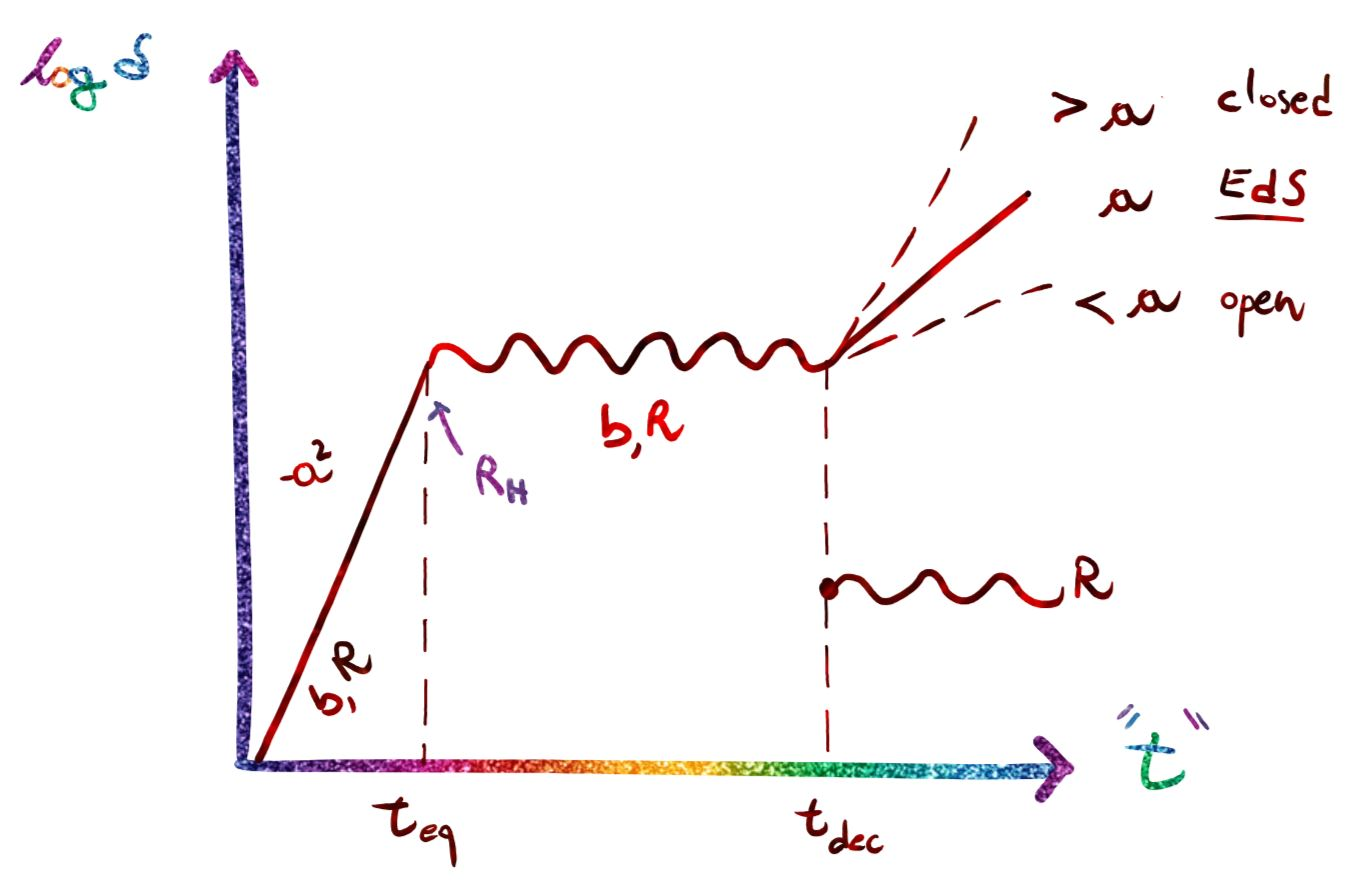
\includegraphics[width=.9 \textwidth]{Pictures/6/growingfactor.jpg}
    \caption{Universo di barioni e radiazione. Non fidarsi delle concavità.}
\end{figure}

\begin{example}[Universo di materia oscura, barioni e radiazione]
Per radiazione e barioni si ripete lo scenario appena visto con $\delta_b,\; \delta_{DM} \bowtie \delta_R$. La materia oscura, dopo l'equivalenza, continua però a crescere come $a$ (è lecitissimo assumere EdS in questo periodo). Questo perché la materia oscura si è già disaccoppiata. Questo fenomeno genera una differenza di altezza fra il contrasto di densità della DM e quello dei barioni, che verrà recuperata a partire da $t_{dec}$ (baryon catch-up). Gli ordini di grandezza di $\delta$ in più (fino 3 dex) rispetto a prima sono un regalo della DM.
[Considerando perturbazioni che entrano nell'orizzonte prima dell'equivalenza, si avrebbero plot leggermente diversi (effetto della stagnazione, ecc...)]
\end{example}


\begin{figure}[ht]
    \centering
    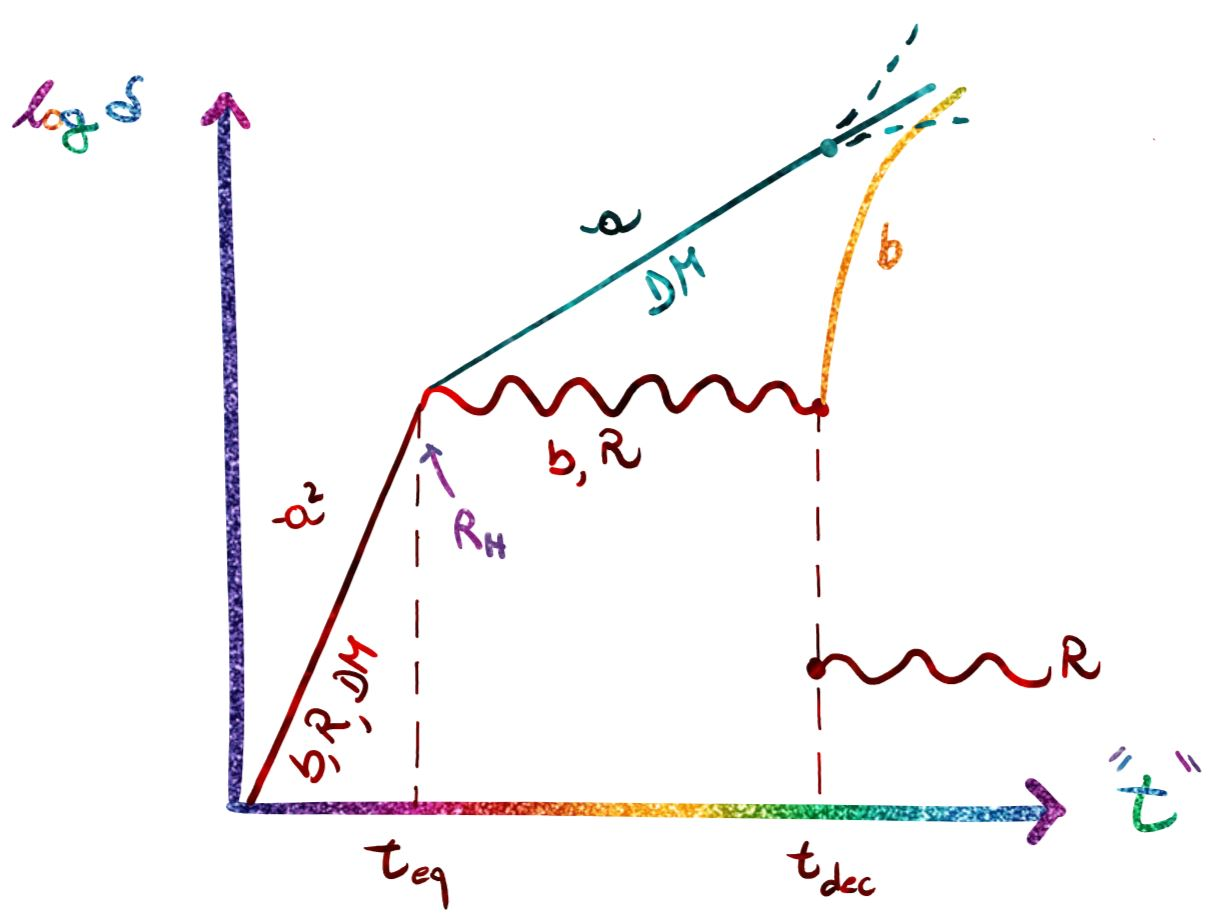
\includegraphics[width=.9 \textwidth]{Pictures/6/dmgrowingfactor.jpg}
    \caption{Universo di materia oscura, barioni e radiazione. Non fidarsi delle concavità.}
\end{figure}


\subsection{Sommario}

\begin{figure}[H]
    \centering
    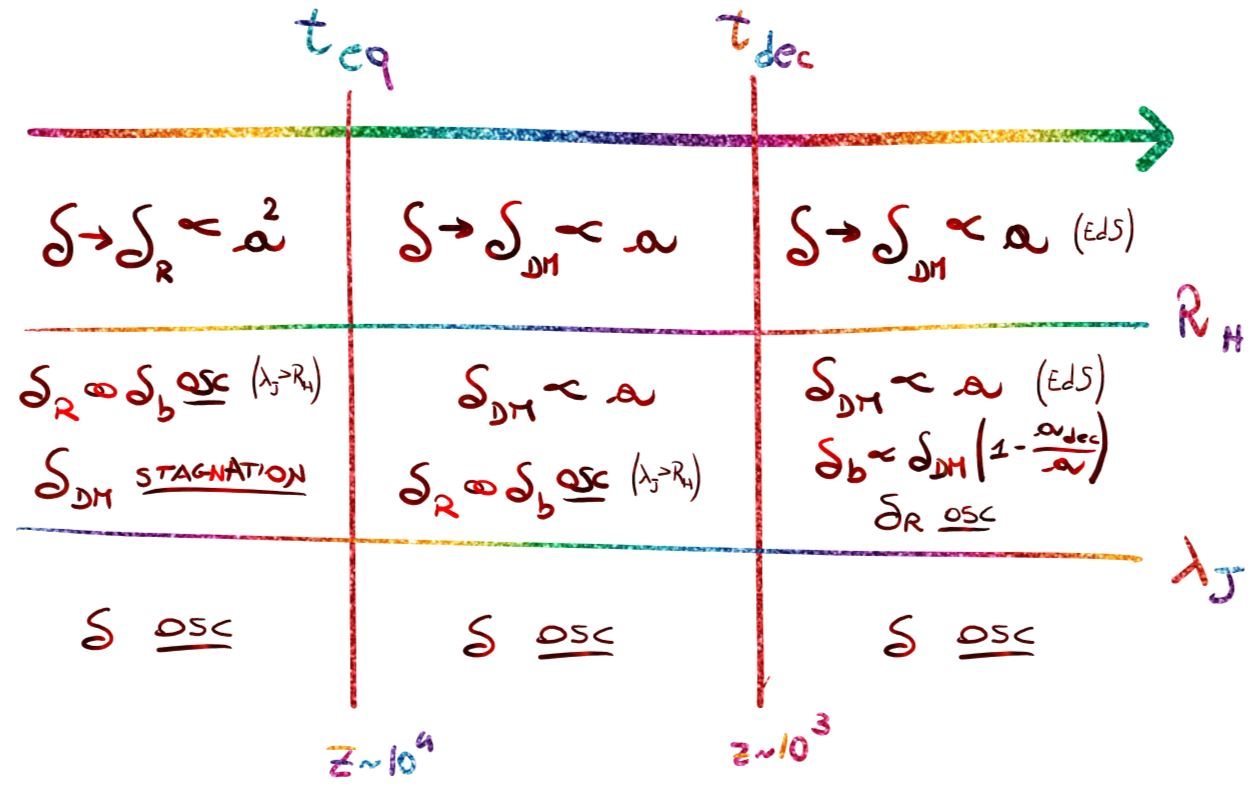
\includegraphics[width=\textwidth]{Pictures/6/sommario.jpg}
    \caption{Riassunto delle soluzioni trovate per il modello di Jeans per un universo in espansione. Mentre per $t<t_{dec}$ è ragionavole aver assunto EdS, la presenza della costante cosmologica può alterare le dipendenza per i tempi successivi ($\delta_{DM}^{close}\propto > a$, $\delta_{DM}^{open}\propto < a$). }
\end{figure}